\documentclass[tikz,border=0.5cm]{standalone}
\everymath{\displaystyle}
\begin{document}
	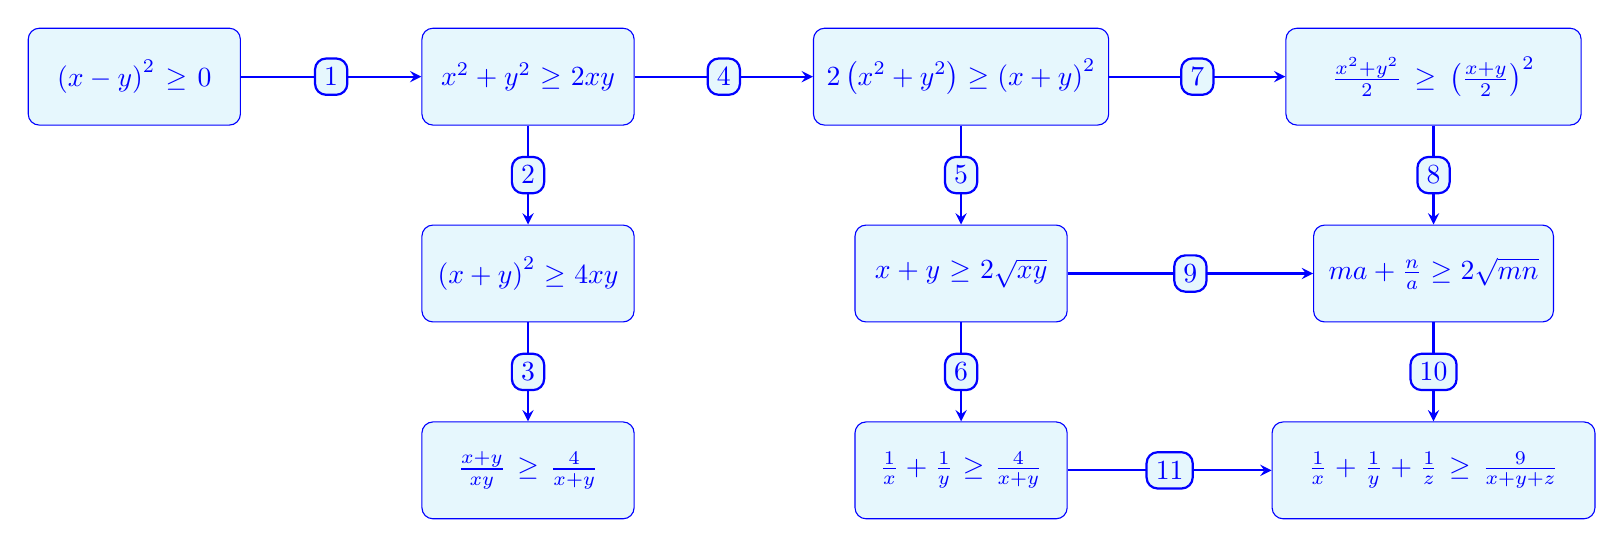
\begin{tikzpicture}[>=stealth,every node/.style={shape=rectangle,draw,rounded corners, color=blue, fill=cyan!10}]
		\tikzstyle{block} = [rectangle, draw, fill=cyan!10, rounded corners, text centered, text width = 7em, minimum height = 3.5em]
		\def\a{5} \def\b{-2.5}
		\path(0,0)node[block](A){$\left( x-y\right)^2 \ge 0$}
		(A)+(\a,0)node[block](B){$x^2 + y^2 \ge 2xy$}
		(B)+(0,\b)node[block](C){$\left( x+y\right) ^2 \ge 4xy$}
		(C)+(0,\b)node[block](D){$\frac{x+y}{xy} \ge \frac{4}{x+y}$}
		(B)+({\a+.5},0)node[block,text width=10em](E){$2\left( x^2+y^2\right) \ge \left( x+y\right)^2$}
		(E)+(0,\b)node[block](F){$x+y \ge 2\sqrt{xy}$}
		(F)+(0,\b)node[block](G){$\frac{1}{x} + \frac{1}{y} \ge \frac{4}{x+y}$}
		(E)+({\a+1},0)node[block,text width=10em](H){$\frac{x^2 + y^2}{2} \ge \left( \frac{x+y}{2}\right)^2$}
		(H)+(0,\b) node[block,text width=8em](I){$ma + \frac{n}{a} \ge 2\sqrt{mn}$}
		(I)+(0,\b) node[block,text width=11em](J){$\frac{1}{x} + \frac{1}{y} + \frac{1}{z}\ge \frac{9}{x+y+z}$};
		\foreach\p/\q [count=\i from 1] in{A/B,B/C,C/D,B/E,E/F,F/G,E/H,H/I,F/I,I/J,G/J}\draw[->,thick,blue](\p)--(\q)node[midway]{\i};
	\end{tikzpicture}
\end{document}